\chapter{Projektplanlægning}\label{Projektplanlaegning}
Dette kapitel vil beskrive hvordan gruppen har planlagt projektforløbet både tidsmæssigt samt opgavemæssigt, og hvilke redskaber vi har benyttet os af til at håndtere planlægningen igennem processen. Således indikere 

\section{Tidsplanlægning}\label{Tidsplanlaegning}
For at optimere vores arbejdsproces bedst muligt og udnytte projektet tiden optimalt muligt, valgte vi at skabe et overblik over hvordan vores tid skulle bruge både på dags-, uge- og månedsbasis, ved hjælp af forskellige redskaber som dagsorden, Trello og Gantt-diagram som havde hvert deres formål igennem 



\subsection{Gantt-diagram}\label{Gantt-diagram}
Efter den første måned af projektarbejdet blev der udviklet et Gantt-diagram, som havde til formål at give et overblik hvordan forventede at vores tid ville blive brugt på de forskellige dele som rapporten skulle indholde. Gantt-diagrammet var tiltænkt at give et estimat på hvordan projektet skulle struktureres, men ikke til at 

\begin{figure}[h]
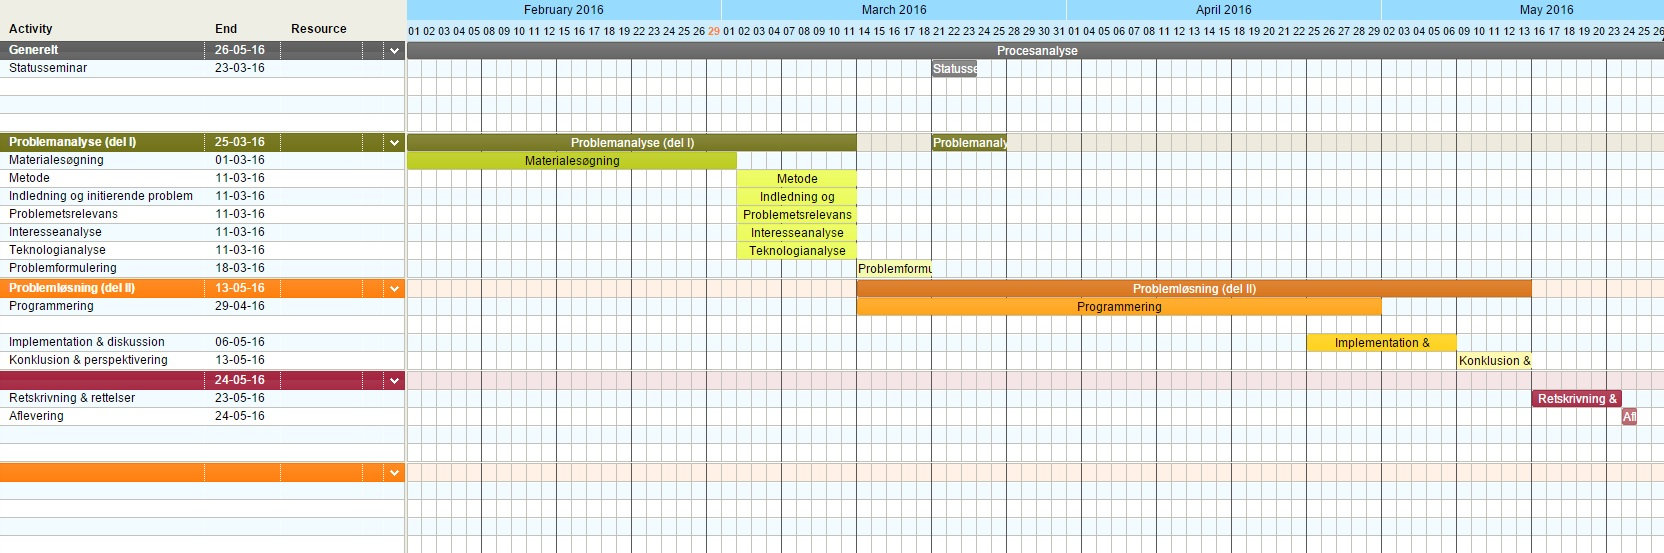
\includegraphics[scale=0.35]{SimuleringGanttdiagramStart}
\centering
\caption{Gruppens første gantt-diagram}\label{Gantt-diagram-picture}
\end{figure}

\section{Opgaveplanlægning}\label{Opgaveplanlaegning}

For at optimere måden at arbejde på og give et overblik over hvad der var hvad blevet færdiggjort og hvad der manglende på dags- og ugebasis, benyttede vi os af dagsorden på tavlen og Trello til at holde styr på projektopgaverne. 

\subsection{Dagsorden}\label{Dagsorden}

Indledende til projektarbejdsdage valgte vi at benytte en dagsorden på tavlen, hvor der blev diskuteret hvad burde være lavet siden sidst, samt om der var skulle tilføjes yderligere opgaver siden sidst. Alle havde til opgave at læse det nye materiale der var blevet skrevet siden sidst, så hvis der var noget der skulle d 

dagsorden blev brugt til at finde ud af hvad der skulle laves og hvad der skulle tilføjes til trello, mens trello blev brugt til at holde styr om opgaverne blev lavet og hvem der gjorde hvad


\subsection{Trello}\label{Trello}
Trello blev brugt som en tilbygning til dagsorden, havde samme formål og bestod hovedsageligt af de samme punkter som inddelt på dagsorden fra tavlen.  over på et elektronisk medie, således at det var muligt at følge med i hvem der var 

\section{Reflektion over projektplanlægningen}\label{Reflektion-over-projektplanlaegningen}
I startfasen hvor alle de forskellige redskaber blev sat op og klar til brug, hvor det var meningen at de skulle benyttes blev de desværre lagt på ro under vores materialesøgning og forsømt indtil midtvejs inde i processen for at sikre at  